%% Section 3 %%%
%\chapter[toc version]{doc version} % эта строка позволяет задать разные названия главы для оглавления и самого документа;


\chapter[Статистическая мощность]{Статистическая мощность и недостаточно мощные статистики}
\chaptermark{Статистическая мощность}% а эта - предписывает название в header на страницах этой главы, http://tex.stackexchange.com/questions/6862/how-can-i-display-a-short-chapter-name-in-the-header-and-a-long-chapter-name-in
\label{chp3}

Мы уже ранее видели, как можно не заметить реальный эффект, взяв недостаточное количество данных. В большинстве случаев это и есть основная проблема: мы можем упустить потенциально действующее лекарство или не заметить серьезный побочный эффект. Как определить, какое количество данных необходимо собрать? 

Отвечая на этот вопрос, статистики используют понятие ``статистическая мощность''. Мощность исследования - это вероятность того, что оно сможет отличить прояление эффекта определенного размера от случайного удачного исхода. Исследование может легко определить огромную пользу какого-либо лекарства, но в меньшей степени способно заметить едва уловимые различия. Давайте рассмотрим простой пример.

Предположим, что игрок убежден в том, что у его оппонента неправильная монета: количество выпадающих орлов и решек у этой монеты отличается от нормального и оппонент этим пользуется, чтобы жульничать в невероятно скучных играх по подбрасыванию монетки. Как это доказать?

Нельзя просто подкинуть монетку 100 раз и подсчитать количество раз, когда выпал орёл. Даже подбрасывая идеальную монетку, вы не всегда получите ровно 50 выпавших орлов: 


\newpage % делаем разрыв, чтобы картинка была первой на след странице

%%%%%%%%%%%%%% figure 1 %%%%%%%%%%%%%%%%%%5
\begin{figure}[h!]
    \centering
    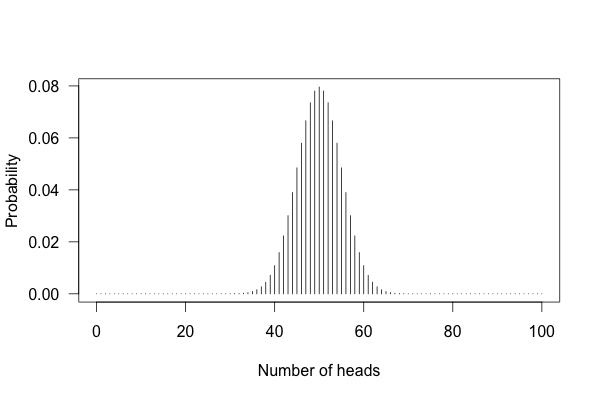
\includegraphics[width=0.8\textwidth]{binomial}
    \caption{На рисунке изображена вероятность (probability) выпадения различного количества орлов (number of heads), если подбросить монетку 100 раз.}
    \label{fig3:binominal}
\end{figure}
%%%%%%%%%%%%%%% end of figure 1 %%%%%%%%%%%%%%%%%%%

Из рисунка видно, что выпавшие 50 раз орлы - это наиболее вероятный исход 100 раз подбрасывания монетки, однако также вполне вероятно и выпадение орла 45 или 57 раз. Если орел выпал 57 раз, причиной тому может быть как неправильная монета, так и просто ваше везение.  

Давайте обратимся к математике. Возьмем, к примеру, \emph{р}-значение равное 0,05 или менее, как обычно делают ученые. То есть, если я посчитаю количество выпавших орлов после 10 или 100 подбрасываний монеты и обнаружу различия с ожидаемым результатом (орел и решка должны выпасть равное количество раз), тогда я смогу назвать монету неправильной, поскольку существует только 5\% шанс получить такое или большее различие, используя нормальную монету. В противном случае, я вообще не могу сделать никакого вывода: может быть монета нормальная, а может быть она немного неправильная, я не могу этого сказать.

Таким образом, что произойдет, если я подброшу монету 10 раз и применю эти рассуждения?


\newpage % делаем разрыв, чтобы картинка была первой на след странице

%%%%%%%%%%%%%% figure 2 %%%%%%%%%%%%%%%%%%5
\begin{figure}[h!]
    \centering
    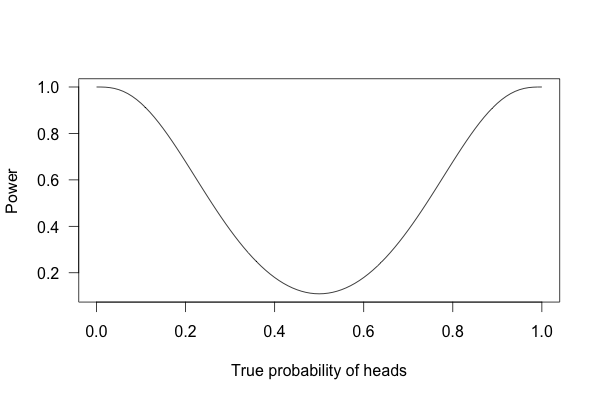
\includegraphics[width=0.8\textwidth]{power-curve-10}
    \caption{Истинная вероятность выпадения орлов}
    \label{fig3:powercurve10}
\end{figure}
%%%%%%%%%%%%%%% end of figure 2 %%%%%%%%%%%%%%%%%%%

Этот рисунок отображает т.н. \emph{функцию мощности}. На горизонтальной оси расположены различные значения, которые может принимать истинная вероятность выпадения орлов, соответствующие разным уровням несправедливости. На вертикальной оси - вероятность того, что я буду считать монету несправедливой (неправильной) после 10 подбрасываний, основываясь на \emph{р}-значении результата.

Можно увидеть, что если монета неправильная и ``подкручена'' на результат в 60\% постоянно выпадающих орлов, а я подбрасываю монету 10 раз, у меня есть лишь 20\% шанс сделать вывод о том, что монета неправильная. В данном случае, у меня слишком мало данных, чтобы отличить неправильную монету от случайности. Чтобы постоянно замечать это, монета должна быть слишком неправильной.

Но что будет, если я подброшу монету 100 раз?

\newpage % делаем разрыв, чтобы картинка была первой на след странице

%%%%%%%%%%%%%% figure 3 %%%%%%%%%%%%%%%%%%5
\begin{figure}[h!]
    \centering
    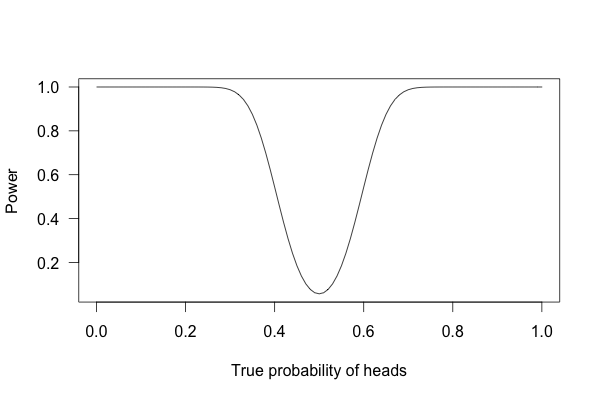
\includegraphics[width=0.8\textwidth]{power-curve-100}
    \caption{Истинная вероятность выпадения орлов}
    \label{fig3:powercurve100}
\end{figure}
%%%%%%%%%%%%%%% end of figure 3 %%%%%%%%%%%%%%%%%%%


А 1000 раз?
%\newpage % делаем разрыв, чтобы картинка была первой на след странице

%%%%%%%%%%%%%% figure 4 %%%%%%%%%%%%%%%%%%5
\begin{figure}[h!]
    \centering
    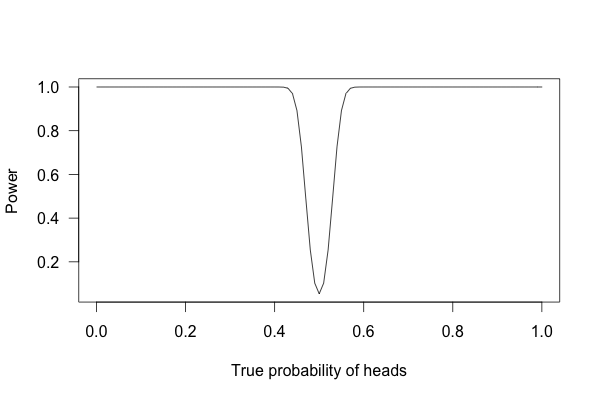
\includegraphics[width=0.8\textwidth]{power-curve-1000}
    \caption{Истинная вероятность выпадения орлов}
    \label{fig3:powercurve1000}
\end{figure}
%%%%%%%%%%%%%%% end of figure 4 %%%%%%%%%%%%%%%%%%%

Подбрасывая монету 1000 раз, я смогу легко понять, ``подкручена'' ли монета на 60\% постоянного выпадения орлов. Крайне маловероятно, что подбрасывая нормальную монету 1000 раз я смогу получить более 600 выпавших орлов.



%%%%%%%%%%%%% new section %%%%%%%%%%%%%%%%%%%%%%%
\section[Недостаточная мощность]{Недостаточная мощность}
\label{chp3:powerunderpowered}

Дочитав до этой строки, у вас может сложится впечатление, что подсчет статистической мощности должен быть неотъемлимой частью клинических испытаний. Учёный, возможно, захочет узнать, какое количество пациентов должно участвовать в испытаниях, при условии, что новое лекарство повышает выживание более чем на 10\%, и он бы получил ответ, быстро рассчитав статистическую мощность. Учёные, обычно, вполне удовлетворены статистической мощностью в 0,8 и более, что соответствует шансу в 80\% сделать вывод о том, что наблюдался реальный эффект. 

Тем не менее, едва ли кто-либо из ученых когда-либо совершал эти подсчеты, и лишь некоторые статьи изредка указывают статистическую мощность используемых тестов.

Давайте рассмотрим эксперимент, направленный на тестирование двух различных лекарств в одинаковых условиях. Вы, возможно, хотели бы узнать, какое из лекарств будет безопаснее, но, к сожалению, побочные эффекты очень редко встречаются. Вы можете протестировать каждое из лекарств на сотнях пациентов, но только у некоторых из них проявятся заметные побочные эффекты.

Естественно, у вас не будет достаточного количества данных, чтобы сравнить оба лекарства по данному критерию: если в одной группе только у 4 пациентов проявились серьезные побочные эффекты, а в другой - только у троих, едва ли вы сможете понять, является ли лекарство причиной их проявлений.


К сожалению, многие эксперименты делают вывод о том, что ``Статистически значимых различий между группами в проявлении побочных эффектов не обнаружено'', не отмечая тот факт, что у них было достаточных данных для обнаружения небольших различий.\cite{tsang_inadequate_2009} И поэтому врачи ошибочно считают, что оба лекарства одинаково безопасны, в то время как одно из них может иметь гораздо опаснее другого.

Можно подумать, что подобная проблема возникает только в ситуациях, когда лекарство имеет слабый эффект, но это не так. В подборке исследований, опубликованных между 1975 и 1990 гг. в престижных медицинских журналах, в 27\% рандомизированных контроллируемых испытаниях были получены отрицательные результаты, но 64\% из них не собрали достаточного количества данных для обнаружения пятидесятипроцентной разницы между тестируемыми группами по основному показателю!!! 50\%!!! Даже если одно из лекарств снижает симптомы на 50\% лучше, чем другое лекарство, данных все равно недостаточно, чтобы признать его более эффективным. И 84\% исследований, получивших отрицательные результаты, не обладали достаточной статистической мощностью, чтобы определить и различия в 25\%. \cite{moher_statistical_1994,bedard_statistical_2007,brown_1987,chung_1998}

В нейронауках, ситуация выглядит гораздо хуже. Предположим, мы соберем в единое данные из множества нейронаучных статей, изучающих один и тот же эффект и уверенно оценивающих размер этого эффекта. Если взять медианное исследование, у него будет только 20\% шанс обнаружить этот эффект. Только после аггрегации множества исследований, данный эффект можно было заметить. Схожие проблемы возникают и в нейронаучных исследованиях, использующих моделирование животных - что формирует значительную этическую проблему: если каждое исследование в отдельности не имеет достаточной статистической мощности, эффект может быть обнаружен только после проведения большого количества исследований (и использования большого количества животных), в то время как можно всего лишь должным образом провести первое исследование.\cite{button_power_2013}

Не говоря уже о том, что ученые лгут, когда заявляют, что они не обнаружили значимых различий между группами. Вы лишь обманываете себя, когда предполагаете, что это означает отсутствие \emph{реальных} различий. Различия могут существовать, но ваше исследование было слишком маленьким, чтобы их заметить.

Вот еще один пример, который мы наблюдаем ежедневно.

\section{Поворот на красный сигнал}
\label{chp3:wrongturnred}

В 1970-х во многих частях США стали разрешать водителям поворачивать направо на красный сигнал светофора. До этого момента, в течении долгого времени проектировщики дорог и инженеры спорили о том, приведёт ли это к увеличению ДТП, в том числе, с участием пешеходов. Но разразившийся в 1973 году нефтяной кризис и его последствия побудили политиков рассматривать вопрос о разрешении поворота на красный сигнал исходя из идеи экономии горючего, которое впустую использовалось, в ожидании разрешающего сигнала светофора. 

Для изучения этого вопроса было проведено несколько исследований. Например, консультант департамента автомагистралей и транспорта Вирджинии провел т.н. ``до и после'' исследование двадцати перекрёстков, на которых разрешили поворот направо на красный сигнал светофора. За примерно одинаковый промежуток времени до разрешения на этих перекрестках произошло 308 ДТП, а после разрешения - 337. Однако, это различие не было статистически значимым, и поэтому консультант сделал вывод, что никакого влияния на безопасность дорожной ситуации разрешение поворота на красный сигнал не имело.

Несколько последующих исследований получили схожие результаты: небольшое увеличение в количестве ДТП, но этих данных было недостаточно для того, чтобы сделать вывод о значимом ухудшении ситуации. Один из отчетов подвел итог таким образом: 

\begin{quotation}
Нет ни единой причины считать, что количество ДТП с участием пешеходов и машин, поворачивающих на красный сигнал светофора направо, увеличилось с момента разрешения поворота направо на красный сигнал\dots
\end{quotation}

Основываясь на этих данных, все больше городов и штатов стали разрешать поворот направо на красный сигнал светофора. Проблема, естественно, заключается в том, что все проводившиеся исследования обладали низкой мощностью. Все большее количество пешеходов были сбиты автомобилями и все большее количество автомобилей участвовало в ДТП, однако никто не мог собрать достаточное количество данных, чтобы убедительно это доказать, до тех пор, пока исследования не стали давать отчетливые результаты: спустя несколько лет стало очевидно значительное увеличение ДТП (в некоторых случаях до 100\%) с участием машин и пешеходов.\cite{hauer_harm_2004,preusser_effect_1982} Такое ошибочное толкование исследований с недостаточной мощностью стоило человеческих жизней.  
